Historii psaní dokumentů jsme si popsali v minulé kapitole, nyní je čas popsat princip, kterým dokumenty vznikají. Vznik dokumentů totiž také prochází
vývojem, ale tento vývoj přichází až v poslední době s rozvojem informačních technologí. Tvorba dokumentů by se dala rozdělit na dva různé přístupy.
Jeden má za výsledek jeden soubor, který tvoří daný dokument a druhý pouze složí dokument z určitých částí.

Než si ovšem popíšeme tyto dva přístupy, je nutné se podívat jak vlastně dokument vzniká. Nejdříve je nutné vytvořit návrh neboli se také používá
označení draft. Tento draft je pouze základní obrys toho co by měl výsledný dokument obsahovat. Pokud se na dokumentu podílí vícero autorů, je
tento draft kontrolován každým z nich. Z draftu se potom začne rozvíjet výsledný dokument, který se po dopsání předává ke kontrole korektorům,
kde se kontroluje pravopis a stylistika. Po konečné kontrole díla autorem či autory je dílo předáno distributorovi. Celý tento postup
je znázorněn na grafu \ref{fig:linflow}

\begin{figure}[h]
    \centering
    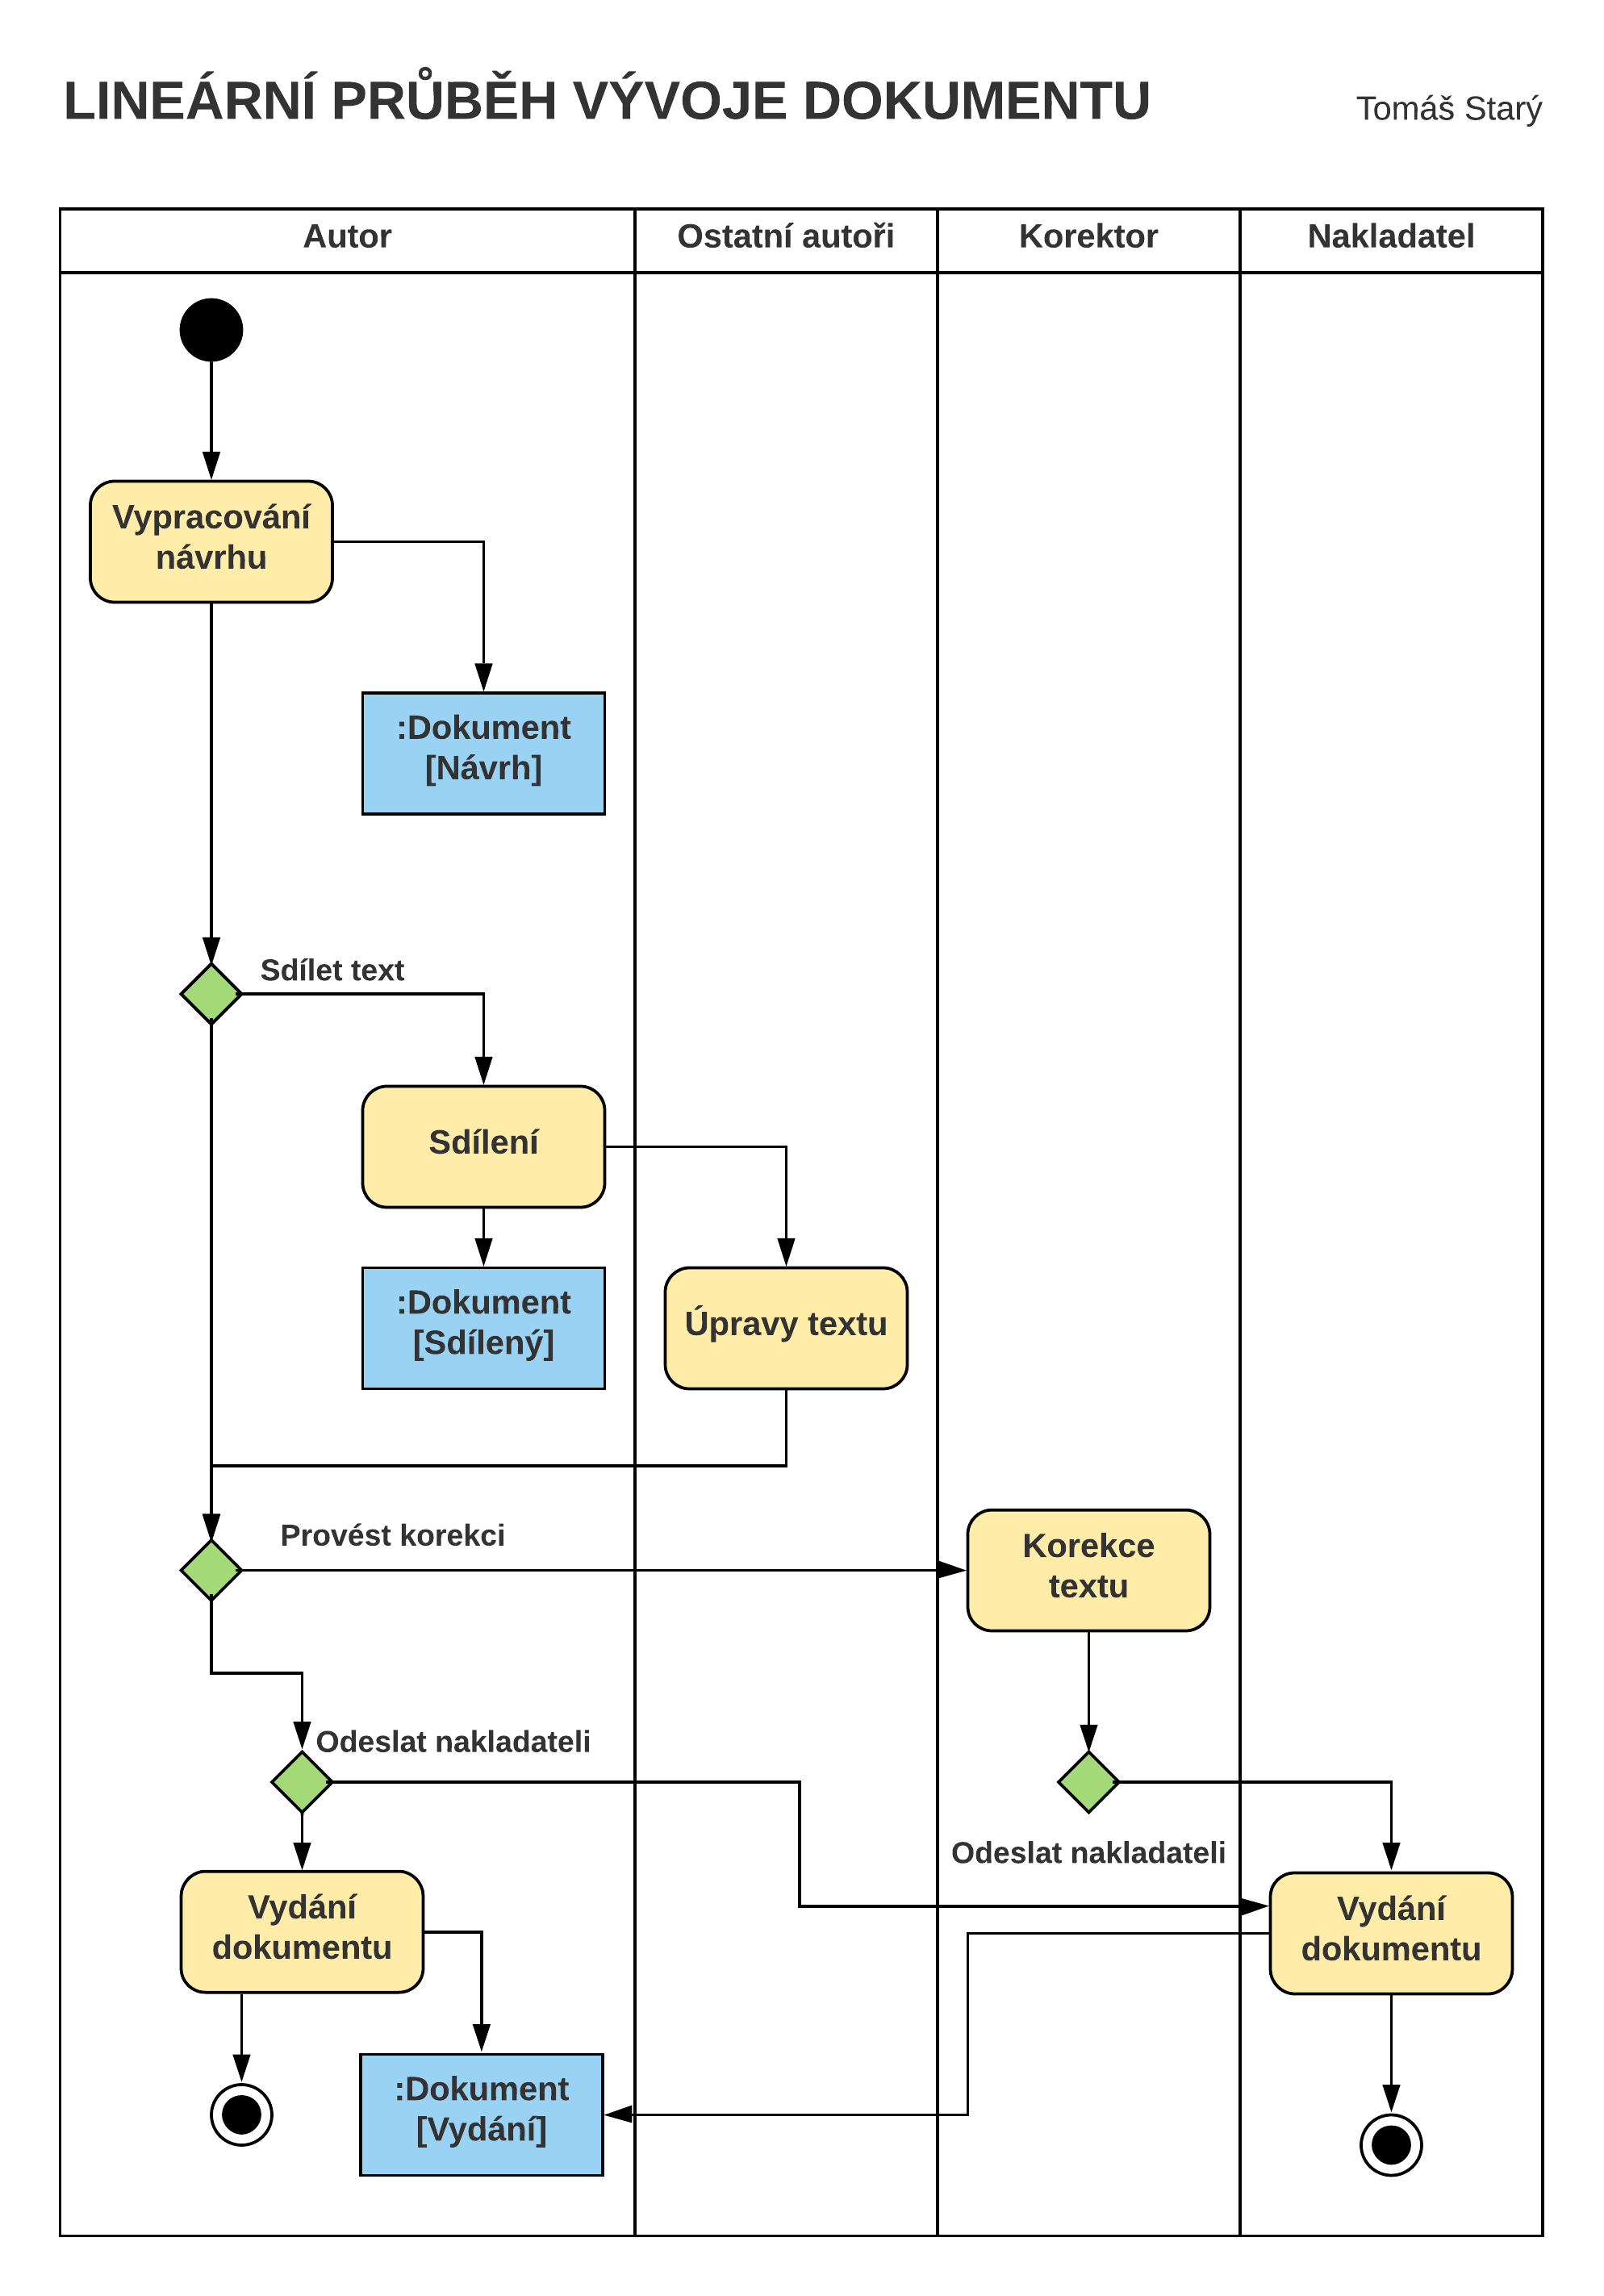
\includegraphics[width=\textwidth]{linearni_prubeh.png}
    \caption{Swimlines diagram}
    \label{fig:linflow}
\end{figure}

\section{Monolitický přístup}

Monolitickým přístupem je myšleno to, že jednotlivé dokumenty jsou jednotné celky, jeden dokument je jeden celek. Pro představu, pokud si vezmeme ku příkladu
Word, o kterém už zaznělo něco v kapitole o historii psaní dokumentů, vytvořením jednoho souboru s příponou .docx, jsme vytvořili jeden monolitický dokument, pokud jej
budeme chtít použít v jiném dokumentu, budeme muset obsah tohoto souboru zkopírovat do nového souboru. Tento nový soubor, který bude obsahovat i náš původní dokument,
pokud se ovšem něco změní v původním dokumentu, druhý dokument bude mít stále původní verzi. Toto poté přináší problémy, které byly již nastíněny v úvodu této práce.

\section{Modulární přístup}

Hlavní myšlenkou modulárních dokumentů je rozdělit dokument na jednotlivé moduly, tedy části textu, které je možné poté využít i v jiných dokumentech. Jako příklad uvedu
tuto práci, skladá se z jednotlivých kapitol. Tyto kapitoly jsou více či méně na sobě nezávislé a tudíž se dají rozdělit na jednotlivé moduly. Ovšem nemusíme tento
dokument dělit pouze podle kapitol, je možné jej rozdělit i na měnší části. S tímto dělením si ovšem musíme dát pozor, abychom dokument nerozdělili na moc malé části,
které potom samy o sobě nebudou mít moc smysl.

Jak nám toto ale pomůže zlepšit efektivitu psaní a rozšiřování dokumentů? Hlavní je si uvědomit, že pokud se například nový člen týmu, který se má starat o nějakou
dokumentaci, má začlenit do jejího psaní a rozšiřování, je velice těžké se orientovat v jednom velkém monolitickém souboru, pokud ovšem je možnost dokumentaci rozdělit
na části, je i pro nově příchozího jednodušší zorientovat se v této části a případně jí upravit. Pro lidi, kteří dokumentaci píšou již delší dobu, bude mimo jiné přínosné
nutnost držet se jednoho tématu, který může definovat daný modul a tím pádem držet konzistentnost textu. \cite{modularDocuments}
